\documentclass{article}
\title{Reading Note 8 for Gaussian Process}
\author{Xiang Pan}

\usepackage{url}
\usepackage{titling}
\usepackage{geometry}
\usepackage{amssymb}

% \geometry{a4paper,scale=0.9,left=10mm, right=10mm, top=3mm, bottom=20mm}
\geometry{a4paper,scale=0.9}
\usepackage{amsmath}
\usepackage{hyperref}
\usepackage{amsfonts}
\usepackage{tikz}
\def\ci{\perp\!\!\!\perp}
\usetikzlibrary{fit,positioning}

\hypersetup{
    colorlinks=true,
    linkcolor=blue,
    filecolor=blue,      
    urlcolor=blue,
    citecolor=cyan,
}


\begin{document}
% \maketitle
\section{GP}
Gaussian processes are mathematically equivalent to many well known models, including Bayesian linear models, spline models, large neural networks (under suitable conditions).

\subsection{weight-space view}
Projecting the inputs into a high-dimensional feature space and applying the linear model there.
\subsection{function-space view}
 Defining a distribution over functions, and inference taking place directly in the space of functions.

 A Gaussian process is a collection of random variables, any finite number of which have a joint Gaussian distribution.

 \begin{equation}
    \begin{aligned}
    m(\mathbf{x}) &=\mathbb{E}[f(\mathbf{x})] \\
    k\left(\mathbf{x}, \mathbf{x}^{\prime}\right) &=\mathbb{E}\left[(f(\mathbf{x})-m(\mathbf{x}))\left(f\left(\mathbf{x}^{\prime}\right)-m\left(\mathbf{x}^{\prime}\right)\right)\right]
    \end{aligned}
\end{equation}

\begin{equation}
    f(\mathbf{x}) \sim \mathcal{G P}\left(m(\mathbf{x}), k\left(\mathbf{x}, \mathbf{x}^{\prime}\right)\right)
\end{equation}

\textbf{Prediction with Noise-free Observations}
\begin{equation}
    \left[\begin{array}{c}
    \mathbf{f} \\
    \mathbf{f}_{*}
    \end{array}\right] \sim \mathcal{N}\left(\mathbf{0},\left[\begin{array}{ll}
    K(X, X) & K\left(X, X_{*}\right) \\
    K\left(X_{*}, X\right) & K\left(X_{*}, X_{*}\right)
    \end{array}\right]\right)
\end{equation}

\textbf{Prediction using Noisy Observations}
\begin{equation}
    \operatorname{cov}\left(y_{p}, y_{q}\right)=k\left(\mathbf{x}_{p}, \mathbf{x}_{q}\right)+\sigma_{n}^{2} \delta_{p q} \text { or } \operatorname{cov}(\mathbf{y})=K(X, X)+\sigma_{n}^{2} I
\end{equation}
\begin{equation}
    \left[\begin{array}{c}
    \mathbf{y} \\
    \mathbf{f}_{*}
    \end{array}\right] \sim \mathcal{N}\left(\mathbf{0},\left[\begin{array}{cc}
    K(X, X)+\sigma_{n}^{2} I & K\left(X, X_{*}\right) \\
    K\left(X_{*}, X\right) & K\left(X_{*}, X_{*}\right)
    \end{array}\right]\right)
\end{equation}
    % \begin{center} 
\begin{figure}[!htp]
    \center
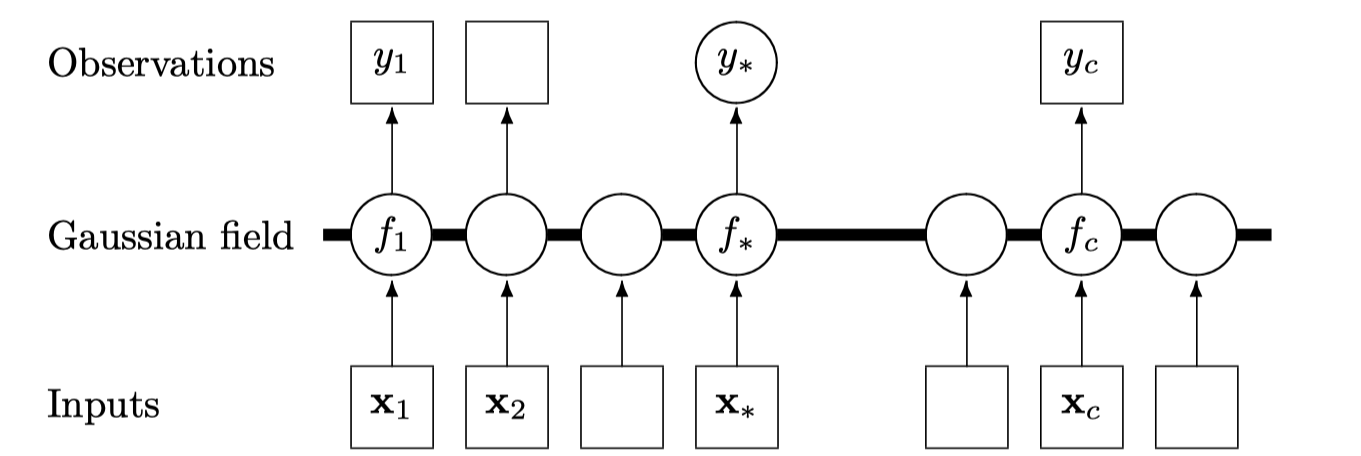
\includegraphics[width=0.5\linewidth]{./images/gp_gm.png}
\caption{Graphical Model for GP}
\end{figure}

\begin{equation}
    \mathbf{f}_{*} \mid X, \mathbf{y}, X_{*} \sim \mathcal{N}\left(\overline{\mathbf{f}}_{*}, \operatorname{cov}\left(\mathbf{f}_{*}\right)\right)
\end{equation}
\begin{equation}
    \overline{\mathbf{f}}_{*} \triangleq \mathbb{E}\left[\mathbf{f}_{*} \mid X, \mathbf{y}, X_{*}\right]=K\left(X_{*}, X\right)\left[K(X, X)+\sigma_{n}^{2} I\right]^{-1} \mathbf{y}
\end{equation}
\begin{equation}
    \operatorname{cov}\left(\mathbf{f}_{*}\right)=K\left(X_{*}, X_{*}\right)-K\left(X_{*}, X\right)\left[K(X, X)+\sigma_{n}^{2} I\right]^{-1} K\left(X, X_{*}\right)
\end{equation}

\begin{equation}
    \begin{aligned}
    \bar{f}_{*} &=\mathbf{k}_{*}^{\top}\left(K+\sigma_{n}^{2} I\right)^{-1} \mathbf{y} \\
    \mathbb{V}\left[f_{*}\right] &=k\left(\mathbf{x}_{*}, \mathbf{x}_{*}\right)-\mathbf{k}_{*}^{\top}\left(K+\sigma_{n}^{2} I\right)^{-1} \mathbf{k}_{*}
    \end{aligned}
\end{equation}



\section{Varying the Hyperparameters}
Of course we can take the position of a quickly-varying signal with low noise, or a slowly-varying signal with high noise to extremes; the former would give rise to a white-noise process model for the signal, while the latter would give rise to a constant signal with added white noise.

\section{Decision Theory for Regression}
In general the value of $y_{\text {guess }}$ that minimizes the risk for the loss function $\mid y_{\text {guess }}-$ $y_{*} \mid$ is the median of $p\left(y_{*} \mid \mathbf{x}_{*}, \mathcal{D}\right)$, while for the squared loss $\left(y_{\text {guess }}-y_{*}\right)^{2}$ it is the mean of this distribution. When the predictive distribution is Gaussian, the mean and the median coincide.


\bibliographystyle{plain}
\bibliography{note8}
\nocite{*}
\appendix
\end{document}